% Bridge Paper 6: Admissible Geometry and Reconstruction Dynamics
% Compile with pdflatex
% Overleaf-ready

\documentclass[11pt]{article}

%=============================================================================
% PACKAGES
%=============================================================================
\usepackage{amsmath,amssymb,amsthm}
\usepackage[margin=1in]{geometry}
\usepackage{hyperref}
\usepackage{graphicx}
\usepackage[dvipsnames]{xcolor}
\usepackage{enumitem}
\usepackage{tikz}
\usetikzlibrary{arrows.meta,shapes,positioning,decorations.pathmorphing,calc}

%=============================================================================
% THEOREM ENVIRONMENTS
%=============================================================================
\theoremstyle{definition}
\newtheorem{definition}{Definition}[section]
\newtheorem{hypothesis}{Hypothesis}[section]

\theoremstyle{plain}
\newtheorem{proposition}{Proposition}[section]
\newtheorem{lemma}{Lemma}[section]
\newtheorem{corollary}{Corollary}[section]

\theoremstyle{remark}
\newtheorem{remark}{Remark}[section]

%=============================================================================
% CUSTOM COMMANDS
%=============================================================================
\newcommand{\Gspace}{\mathcal{G}}
\newcommand{\Mfunc}{\mathcal{M}}
\newcommand{\Rmap}{\mathcal{R}}
\newcommand{\Egeom}{E_{\mathrm{geom}}}
\newcommand{\Meff}{M_{\mathrm{eff}}}
\newcommand{\Adm}{\mathcal{A}}
\newcommand{\dd}{\mathrm{d}}

%=============================================================================
% HYPERREF SETUP
%=============================================================================
\hypersetup{
    colorlinks=true,
    linkcolor=blue!70!black,
    citecolor=green!50!black,
    urlcolor=blue!70!black
}

%=============================================================================
% TITLE
%=============================================================================
\title{\textbf{Bridge Paper 6: Admissible Geometry and Reconstruction Dynamics}\\[0.5em]
\large\textit{First Draft --- December 4, 2025}}

\author{Lee Smart\\[0.6em]
\textit{Vibrational Field Dynamics Institute}\\[0.3em]
Email: \texttt{contact@vibrationalfielddynamics.org}\\
X (Twitter): \texttt{@vfd\_org}\\
Website: \texttt{https://vfd.org}}

\date{December 4, 2025}

%=============================================================================
\begin{document}
%=============================================================================

\maketitle

%-----------------------------------------------------------------------------
% ABSTRACT
%-----------------------------------------------------------------------------
\begin{abstract}
Bridge Paper~5 (BP5) established that apparent motion of localised field configurations
can be reinterpreted as sequential reconstruction: a time-indexed family of stabilised
geometries related by reconstruction maps, rather than literal transport of objects
through space. The present paper elevates this reconstruction picture from an
interpretive framework to a \emph{selection principle}. We define the configuration
space~$\Gspace$ of stabilised geometries and formulate admissibility constraints---stability,
bounded mismatch, and internal mode regularity---that filter which reconstruction
sequences are physically allowed. Dynamics thus emerges not as forces acting on objects,
but as constrained selection within~$\Gspace$: admissible histories are selected
by reconstruction constraints, not generated by equations of motion. In the deep-stabilisation and slow-evolution regime,
we show that admissible paths approximate geodesics on a metric inherited from the
mismatch functional, recovering the effective mass and kinetic structure of BP4.
Multi-configuration systems introduce constraint coupling, which yields effective
interaction potentials in the infrared limit. Conservation laws arise from symmetries
of the admissibility conditions. We explicitly delineate the regime of validity and
enumerate claims that this framework does not make.

\medskip
\noindent\textbf{Status:} First public draft. Comments welcome.
\end{abstract}

\tableofcontents

\newpage

%=============================================================================
\section{Introduction: From Interpretation to Selection}
\label{sec:introduction}
%=============================================================================

%-----------------------------------------------------------------------------
\subsection{Recap of BP4 and BP5}
\label{sec:recap}
%-----------------------------------------------------------------------------

Bridge Paper~4 (BP4)~\cite{BP4} demonstrated that a localised, stabilised field
configuration~$\Phi_0$ possesses an effective mass~$\Meff$ derived from the moduli
space metric of the underlying field theory. Slow collective motion along translation
modes yields an effective kinetic energy
\begin{equation}
\label{eq:kinetic-BP4}
T_{\mathrm{eff}} = \frac{1}{2}\Meff \dot{X}^2,
\end{equation}
where $X(t)$ is the collective coordinate labelling the configuration's spatial
localisation. Interactions between well-separated configurations produce effective
potentials, and in the weak-field limit, the Newtonian structure is recovered.

Bridge Paper~5 (BP5)~\cite{BP5} reinterpreted~$X(t)$ not as the literal position of
a transported object, but as a \emph{reconstruction label}: at each instant, the
field is independently stabilised as a geometry~$\Phi_0(X(t))$, and sequential
geometries are related by a reconstruction map~$\Rmap_\Delta$ with mismatch
functional~$\Mfunc$. Motion is thus reconstruction; apparent transport is the
time-ordered correspondence between stable configurations.

%-----------------------------------------------------------------------------
\subsection{The Selection Problem}
\label{sec:selection-problem}
%-----------------------------------------------------------------------------

BP5 provides an interpretation of what motion \emph{is}, but does not specify
\emph{which} reconstruction sequences are allowed. The reconstruction map~$\Rmap_\Delta$
relates consecutive geometries, and the mismatch~$\Mfunc$ quantifies their difference,
yet infinitely many sequences~$\{\gamma_k\}$ could in principle be constructed.
The \textbf{selection problem} is: what determines the admissible set of reconstruction
histories?

This paper answers that question by formulating \emph{admissibility constraints}
on histories in the configuration space of stabilised geometries. Dynamics is
thereby recast as selection: the physically realised history is one (or one among
few) that satisfies all constraints.

%-----------------------------------------------------------------------------
\subsection{Goal of BP6}
\label{sec:goal}
%-----------------------------------------------------------------------------

The goal of this paper is to:
\begin{enumerate}[label=(\roman*)]
    \item Define the configuration space~$\Gspace$ of stabilised geometries and
          the space of histories over~$\Gspace$.
    \item Formulate admissibility constraints---stability, bounded mismatch,
          internal mode regularity---as precise mathematical conditions.
    \item Show that admissible evolution under these constraints yields, in the
          appropriate regime, the geodesic/inertial structure recovered in BP4/BP5.
    \item Demonstrate that multi-configuration constraint coupling produces
          effective interactions.
\end{enumerate}

BP5 resolved the \emph{interpretation} of motion; BP6 specifies \emph{admissibility
and selection}.

%-----------------------------------------------------------------------------
\subsection{Conceptual Dictionary}
\label{sec:dictionary}
%-----------------------------------------------------------------------------

To orient the reader, Table~\ref{tab:dictionary} contrasts standard dynamical
language with the admissibility-based vocabulary employed here.

\begin{table}[h]
\centering
\caption{Conceptual dictionary: transport/force language versus admissibility/constraint
language.}
\label{tab:dictionary}
\begin{tabular}{ll}
\hline
\textbf{Standard Dynamics} & \textbf{Admissibility Framework (BP6)} \\
\hline
Object/particle & Stabilised geometry $\gamma \in \Gspace$ \\
Position $X(t)$ & Collective coordinate / reconstruction label \\
Trajectory & Admissible history in $\Gspace$ \\
Force & Constraint coupling gradient \\
Acceleration & Deviation of admissible path from free geodesic \\
Inertia & Mismatch cost for configuration change \\
Potential energy & Constraint-induced effective energy \\
Equation of motion & Admissibility selection rule \\
\hline
\end{tabular}
\end{table}

%=============================================================================
\section{Configuration Space of Stabilised Geometry}
\label{sec:config-space}
%=============================================================================

%-----------------------------------------------------------------------------
\subsection{Field Configurations and Stabilised Minima}
\label{sec:field-config}
%-----------------------------------------------------------------------------

We work with a real scalar field~$\Phi: \mathbb{R}^3 \times \mathbb{R} \to \mathbb{R}$,
though the framework extends to more general field content. The energy functional is
\begin{equation}
\label{eq:energy-functional}
E[\Phi] = \int_{\mathbb{R}^3} \dd^3 x \left[
    \frac{1}{2c^2}(\partial_t \Phi)^2 + \frac{1}{2}(\nabla \Phi)^2 + V(\Phi)
\right],
\end{equation}
where $V(\Phi)$ is a potential admitting localised, stable minima. The gradient
energy~$\Egeom[\Phi]$ is defined by
\begin{equation}
\label{eq:Egeom}
\Egeom[\Phi] \;=\; \int_{\mathbb{R}^3} \dd^3 x \left[
    \frac{1}{2}(\nabla \Phi)^2 + V(\Phi)
\right].
\end{equation}
A \textbf{stabilised configuration} is a static or quasi-static field profile~$\Phi_0$
satisfying
\begin{equation}
\label{eq:stable-condition}
\frac{\delta \Egeom}{\delta \Phi}\bigg|_{\Phi_0} = 0, \qquad
\text{with positive-definite second variation (modulo zero modes)}.
\end{equation}

\begin{definition}[Stabilised Geometry]
\label{def:stabilised-geom}
A \emph{stabilised geometry}~$\gamma$ is an equivalence class~$[\Phi_0]$ of
stabilised configurations related by spatial translations and any internal
symmetry transformations of the field theory.
\end{definition}

The equivalence removes redundancy: two configurations differing only by a global
translation represent the same intrinsic geometry.

%-----------------------------------------------------------------------------
\subsection{The Configuration Space \texorpdfstring{$\Gspace$}{G}}
\label{sec:Gspace}
%-----------------------------------------------------------------------------

\begin{definition}[Configuration Space]
\label{def:config-space}
The \emph{configuration space of stabilised geometries} is
\begin{equation}
\label{eq:Gspace}
\Gspace \;=\; \bigl\{ \gamma = [\Phi_0] : \Phi_0 \text{ satisfies }
\eqref{eq:stable-condition} \bigr\} \big/ \sim,
\end{equation}
where $\sim$ denotes the equivalence under spatial translations and internal symmetries.
\end{definition}

Elements of~$\Gspace$ are not ``particles at positions'' but intrinsic stable
field geometries. A representative~$\Phi_0(x; q)$, parameterised by collective
coordinates~$q = (X, \xi)$---where $X \in \mathbb{R}^3$ labels translation and
$\xi$ labels internal moduli---can be chosen for computational purposes, but
the physical object is the equivalence class.

Figure~\ref{fig:config-space} illustrates the structure of~$\Gspace$.

\begin{figure}[ht]
\centering
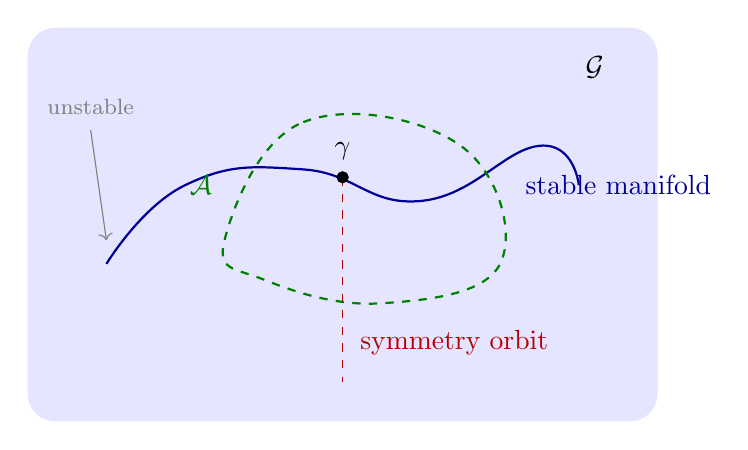
\begin{tikzpicture}[scale=1.0]
    % Shaded region for G
    \fill[blue!10, rounded corners=10pt] (-3,-2) rectangle (5,3);
    \node at (4.2,2.5) {$\Gspace$};

    % Stable manifold
    \draw[thick, blue!60!black] plot[smooth, tension=0.8]
        coordinates {(-2,0) (-1,1) (0.5,1.2) (2,0.8) (3.5,1.5) (4,1)};
    \node[blue!60!black] at (4.5,1) {stable manifold};

    % Symmetry orbit (vertical fiber)
    \draw[dashed, red!70!black] (1,1.1) -- (1,-1.5);
    \node[red!70!black, right] at (1.1,-1) {symmetry orbit};

    % Point gamma
    \filldraw[black] (1,1.1) circle (2pt);
    \node[above] at (1,1.2) {$\gamma$};

    % Admissible region
    \draw[thick, green!50!black, dashed]
        plot[smooth cycle, tension=0.7]
        coordinates {(-0.5,0.3) (0.5,1.8) (2.5,1.5) (3,0) (1.5,-0.5) (0,-0.2)};
    \node[green!50!black] at (-0.8,1) {$\Adm$};

    % Unstable region indicator
    \node[gray] at (-2.2,2) {\footnotesize unstable};
    \draw[->, gray] (-2.2,1.7) -- (-2,0.3);
\end{tikzpicture}
\caption{Schematic of the configuration space~$\Gspace$ of stabilised geometries.
The stable manifold (solid curve) contains configurations satisfying~\eqref{eq:stable-condition}.
Symmetry orbits (dashed vertical lines) are quotiented out. The admissible
region~$\Adm$ (dashed boundary) is defined by constraints in Section~\ref{sec:admissibility}.}
\label{fig:config-space}
\end{figure}

%-----------------------------------------------------------------------------
\subsection{Histories in \texorpdfstring{$\Gspace$}{G}}
\label{sec:histories}
%-----------------------------------------------------------------------------

\begin{definition}[Discrete History]
\label{def:discrete-history}
A \emph{discrete history} is a sequence $\{\gamma_k\}_{k=0}^{N}$ with
$\gamma_k \in \Gspace$ for each~$k$, indexed by discrete parameter~$k$
corresponding to reconstruction steps of duration~$\Delta$.
\end{definition}

\begin{definition}[Continuous History]
\label{def:continuous-history}
A \emph{continuous history} is a smooth curve $\gamma: [0,T] \to \Gspace$,
$t \mapsto \gamma(t)$.
\end{definition}

The discrete formulation is primary; the continuous limit is derived in
Section~\ref{sec:emergent-inertial} and Appendix~\ref{app:discrete-continuous}.

%-----------------------------------------------------------------------------
\subsection{Observables on \texorpdfstring{$\Gspace$}{G}}
\label{sec:observables}
%-----------------------------------------------------------------------------

Physical observables are functionals $\mathcal{O}: \Gspace \to \mathbb{R}$
invariant under the equivalence relation. Examples include:
\begin{itemize}
    \item Geometric energy: $\Egeom(\gamma)$.
    \item Internal mode amplitudes: projections onto non-translational eigenmodes
          of the stability operator.
\end{itemize}
We do not develop the theory of observables further here; it suffices that
well-defined functionals on~$\Gspace$ exist.

%=============================================================================
\section{Reconstruction Admissibility}
\label{sec:admissibility}
%=============================================================================

%-----------------------------------------------------------------------------
\subsection{The Reconstruction Map}
\label{sec:recon-map}
%-----------------------------------------------------------------------------

Following BP5~\cite{BP5}, we define a reconstruction map that relates consecutive
geometries in a discrete history.

\begin{definition}[Reconstruction Map]
\label{def:recon-map}
The \emph{reconstruction map} $\Rmap_\Delta: \Gspace \to \Gspace$ associates to
each stabilised geometry~$\gamma_k$ a candidate successor geometry~$\Rmap_\Delta(\gamma_k)$,
representing the ``natural continuation'' under reconstruction at time-step~$\Delta$.
\end{definition}

The precise form of~$\Rmap_\Delta$ depends on the dynamics of the underlying field
theory. For present purposes, it suffices that $\Rmap_\Delta$ encodes the tendency
of a configuration to persist or evolve according to intrinsic field dynamics
over one reconstruction step.

%-----------------------------------------------------------------------------
\subsection{The Mismatch Functional}
\label{sec:mismatch}
%-----------------------------------------------------------------------------

\begin{definition}[Mismatch Functional]
\label{def:mismatch}
The \emph{mismatch functional} $\Mfunc: \Gspace \times \Gspace \to \mathbb{R}_{\geq 0}$
quantifies the discrepancy between two geometries:
\begin{equation}
\label{eq:mismatch}
\Mfunc(\gamma', \gamma; \Rmap) \;=\;
\inf_{\substack{\Phi_0 \in \gamma \\ \Phi_0' \in \gamma'}}
\int_{\mathbb{R}^3} \dd^3x \, \bigl| \Phi_0'(x) - \Rmap_\Delta[\Phi_0](x) \bigr|^2
\, w(x),
\end{equation}
where $w(x) \geq 0$ is a weight function (e.g., $w = 1$ or localised to the
configuration's support), and the infimum is over representatives in each
equivalence class.
\end{definition}

The mismatch measures how well~$\gamma'$ matches the natural successor
$\Rmap_\Delta(\gamma)$. A small mismatch indicates that the transition
$\gamma \to \gamma'$ is consistent with the reconstruction dynamics; a large
mismatch indicates a ``jump'' that reconstruction cannot naturally produce.

%-----------------------------------------------------------------------------
\subsection{Admissibility Constraints}
\label{sec:constraints}
%-----------------------------------------------------------------------------

We now define the constraints that filter admissible histories.

\begin{hypothesis}[Stability Constraint]
\label{hyp:stability}
Each geometry in an admissible history must lie on the stable manifold:
\begin{equation}
\label{eq:stability-constraint}
\gamma_k \in \Gspace_{\mathrm{stable}} \;:\;
\Egeom(\gamma_k) \leq E^* \quad \text{and} \quad
\delta^2 \Egeom|_{\gamma_k} > 0 \; (\text{mod zero modes}).
\end{equation}
\end{hypothesis}

\begin{hypothesis}[Bounded Mismatch]
\label{hyp:bounded-mismatch}
The mismatch between consecutive geometries is bounded:
\begin{equation}
\label{eq:mismatch-bound}
\Mfunc(\gamma_{k+1}, \gamma_k; \Rmap) \;\leq\; \Mfunc^*,
\end{equation}
where $\Mfunc^* > 0$ is a threshold set by the reconstruction fidelity.
\end{hypothesis}

\begin{hypothesis}[Internal Mode Regularity]
\label{hyp:internal-mode}
Excitation of internal (non-collective) modes is bounded:
\begin{equation}
\label{eq:internal-bound}
\bigl\| P_{\mathrm{int}} \delta\gamma_k \bigr\| \;\leq\; \epsilon_{\mathrm{int}},
\end{equation}
where $P_{\mathrm{int}}$ projects onto internal mode directions and
$\delta\gamma_k = \gamma_{k+1} - \gamma_k$ in a suitable linearisation.
\end{hypothesis}

\begin{definition}[Admissible History]
\label{def:admissible-history}
A discrete history $\{\gamma_k\}_{k=0}^N$ is \emph{admissible} if it satisfies
Hypotheses~\ref{hyp:stability}--\ref{hyp:internal-mode} at every step~$k$.
We write $\{\gamma_k\} \in \Adm$.

A continuous history $\gamma(t)$ is admissible if it is the $\Delta \to 0$ limit
of admissible discrete histories (see Appendix~\ref{app:discrete-continuous}).
\end{definition}

Figure~\ref{fig:admissible-update} illustrates the discrete admissible update.

\begin{figure}[ht]
\centering
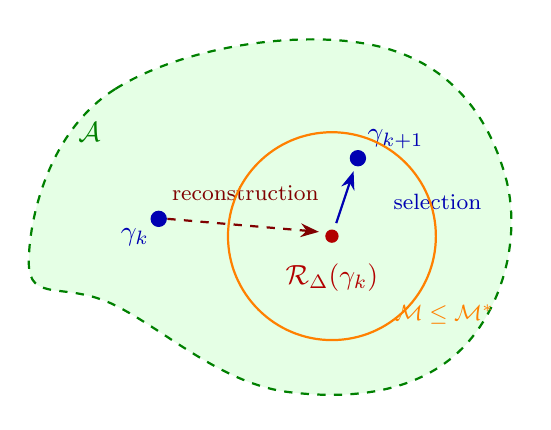
\begin{tikzpicture}[scale=1.1]
    % Admissible region
    \fill[green!10] plot[smooth cycle, tension=0.7]
        coordinates {(-1,0) (0,2) (3,2.5) (4.5,1) (4,-1) (2,-1.5) (0,-0.5)};
    \draw[thick, green!50!black, dashed] plot[smooth cycle, tension=0.7]
        coordinates {(-1,0) (0,2) (3,2.5) (4.5,1) (4,-1) (2,-1.5) (0,-0.5)};
    \node[green!50!black] at (-0.3,1.5) {$\Adm$};

    % gamma_k
    \filldraw[blue!70!black] (0.5,0.5) circle (2.5pt);
    \node[blue!70!black, below left] at (0.5,0.5) {$\gamma_k$};

    % R_Delta(gamma_k) - possibly outside admissible
    \filldraw[red!70!black] (2.5,0.3) circle (2pt);
    \node[red!70!black, below] at (2.5,0.1) {$\Rmap_\Delta(\gamma_k)$};

    % Arrow from gamma_k to R_Delta
    \draw[-{Stealth}, thick, red!50!black, dashed] (0.6,0.5) -- (2.35,0.35);
    \node[red!50!black, above] at (1.5,0.6) {\footnotesize reconstruction};

    % gamma_{k+1} - projected/selected
    \filldraw[blue!70!black] (2.8,1.2) circle (2.5pt);
    \node[blue!70!black, above right] at (2.8,1.2) {$\gamma_{k+1}$};

    % Arrow from R_Delta to gamma_{k+1}
    \draw[-{Stealth}, thick, blue!70!black] (2.55,0.45) -- (2.75,1.05);
    \node[blue!70!black, right] at (3.1,0.7) {\footnotesize selection};

    % Mismatch bound circle
    \draw[orange, thick] (2.5,0.3) circle (1.2);
    \node[orange] at (3.8,-0.6) {\footnotesize $\Mfunc \leq \Mfunc^*$};
\end{tikzpicture}
\caption{Discrete admissible update. Starting from~$\gamma_k$, reconstruction
suggests~$\Rmap_\Delta(\gamma_k)$. The admissible successor~$\gamma_{k+1}$ is
selected within the admissible region~$\Adm$ and the mismatch bound (orange circle).}
\label{fig:admissible-update}
\end{figure}

%=============================================================================
\section{Constraints as Selection Rules}
\label{sec:selection-rules}
%=============================================================================

%-----------------------------------------------------------------------------
\subsection{Core Postulate: Admissible Evolution via Constrained Selection}
\label{sec:core-postulate}
%-----------------------------------------------------------------------------

We now state the central postulate of this paper.

\begin{hypothesis}[Selection Principle]
\label{hyp:selection}
Physical evolution corresponds to admissible histories. At each step, the
successor geometry is determined by constrained selection within~$\Adm$.
\end{hypothesis}

We provide two equivalent formulations of this selection.

\paragraph{Formulation (A): Constrained Minimisation.}
The successor geometry minimises the mismatch subject to admissibility:
\begin{equation}
\label{eq:constrained-min}
\gamma_{k+1} = \operatornamewithlimits{argmin}_{\gamma' \in \Adm}
\Mfunc(\gamma', \gamma_k; \Rmap).
\end{equation}

\paragraph{Formulation (B): Feasibility Projection.}
The successor geometry is the admissible point closest to the unconstrained
reconstruction:
\begin{equation}
\label{eq:feasibility-proj}
\gamma_{k+1} = \Pi_{\Adm}\bigl( \Rmap_\Delta(\gamma_k) \bigr),
\end{equation}
where $\Pi_{\Adm}$ denotes projection onto the admissible set with respect
to the metric induced by~$\Mfunc$.

Under regularity conditions (convexity of~$\Adm$ in local coordinates,
smoothness of~$\Mfunc$), these formulations are equivalent.
Both are computational implementations of a selection rule, not fundamental
equations of motion; neither minimisation nor projection is ontologically primitive.

%-----------------------------------------------------------------------------
\subsection{Selection on \texorpdfstring{$\Gspace$}{G}, Not Forces on Objects}
\label{sec:not-forces}
%-----------------------------------------------------------------------------

The selection rule~\eqref{eq:constrained-min} or~\eqref{eq:feasibility-proj}
operates on the configuration space~$\Gspace$, not on ``objects in space.''
There is no force pushing a particle; rather, the admissibility constraints
filter which reconstruction sequences are realised. The language of ``forces''
and ``acceleration'' is recovered only in the effective description
(Section~\ref{sec:emergent-inertial}).

\begin{remark}
This is analogous to the principle of least action: the trajectory is not
``pushed'' by forces instant-by-instant, but selected as the extremum of an
action functional over the entire path space. Here, selection is by
admissibility rather than action extremisation.
\end{remark}

%-----------------------------------------------------------------------------
\subsection{Well-Posedness of the Selection Rule}
\label{sec:well-posed}
%-----------------------------------------------------------------------------

\begin{proposition}[Existence and Uniqueness]
\label{prop:well-posed}
Suppose:
\begin{enumerate}[label=(\alph*)]
    \item $\Adm \subset \Gspace$ is non-empty, closed, and convex in local
          coordinates.
    \item $\Mfunc(\cdot, \gamma_k; \Rmap)$ is continuous and coercive
          on~$\Gspace$.
    \item $\Rmap_\Delta(\gamma_k) \in \Gspace$ for all~$\gamma_k \in \Adm$.
\end{enumerate}
Then the selection rule~\eqref{eq:constrained-min} admits a unique solution
$\gamma_{k+1} \in \Adm$, and the map $\gamma_k \mapsto \gamma_{k+1}$ is continuous.
\end{proposition}

\begin{proof}
Continuity and coercivity of~$\Mfunc$ ensure that the infimum is attained on
the closed set~$\Adm$. Strict convexity of~$\Mfunc$ (inherited from the
$L^2$-type structure in~\eqref{eq:mismatch}) guarantees uniqueness. Continuity
of the update map follows from the maximum theorem.
\end{proof}

%=============================================================================
\section{Emergent Inertial Structure as Extremal Admissibility}
\label{sec:emergent-inertial}
%=============================================================================

%-----------------------------------------------------------------------------
\subsection{Continuous-Time Limit of the Mismatch}
\label{sec:continuous-limit}
%-----------------------------------------------------------------------------

We derive the continuous-time limit of the mismatch functional. Let
$q = (q^1, \ldots, q^n)$ be local coordinates on~$\Gspace$ (collective coordinates
for the configuration). Over a time step~$\Delta$, write
\begin{equation}
\label{eq:q-expansion}
q_{k+1} = q_k + \dot{q}_k \Delta + O(\Delta^2).
\end{equation}

\begin{proposition}[Mismatch Expansion]
\label{prop:mismatch-expansion}
Under the assumption that $\Rmap_\Delta$ implements free propagation to
leading order, the mismatch functional admits the expansion
\begin{equation}
\label{eq:mismatch-expansion}
\Mfunc(\gamma_{k+1}, \gamma_k; \Rmap) \;=\;
\frac{\Delta}{2} g_{ij}(q) \dot{q}^i \dot{q}^j + O(\Delta^2),
\end{equation}
where $g_{ij}(q)$ is a positive-definite metric on~$\Gspace$ given by
\begin{equation}
\label{eq:metric-def}
g_{ij}(q) \;=\; \int_{\mathbb{R}^3} \dd^3x \,
\frac{\partial \Phi_0}{\partial q^i} \frac{\partial \Phi_0}{\partial q^j} \, w(x).
\end{equation}
\end{proposition}

\begin{proof}
See Appendix~\ref{app:discrete-continuous}.
\end{proof}

The metric~\eqref{eq:metric-def} is precisely the moduli space metric familiar
from soliton dynamics~\cite{Manton1982, Rajaraman1982}. In the translation sector,
$q = X$, and
\begin{equation}
\label{eq:translation-metric}
g_{XX} = \int_{\mathbb{R}^3} \dd^3x \, |\nabla \Phi_0|^2 = \Meff c^2,
\end{equation}
recovering the effective mass of BP4~\cite{BP4}.

%-----------------------------------------------------------------------------
\subsection{Geodesic Structure in the Deep-Stabilisation Regime}
\label{sec:geodesic}
%-----------------------------------------------------------------------------

\begin{definition}[Deep-Stabilisation Regime]
\label{def:deep-stab}
The \emph{deep-stabilisation regime} is the parameter domain where:
\begin{enumerate}[label=(\roman*)}
    \item Internal modes are suppressed: $\| P_{\mathrm{int}} \delta\gamma \| \ll 1$.
    \item Evolution is slow: $|\dot{q}| \Delta \ll \ell$, where $\ell$ is the
          characteristic scale.
    \item Mismatch is small: $\Mfunc \ll \Mfunc^*$.
\end{enumerate}
\end{definition}

In this regime, the admissibility constraints are not saturated, and the
evolution is determined by minimising the mismatch.

\begin{proposition}[Geodesic Approximation]
\label{prop:geodesic}
In the deep-stabilisation regime, admissible paths $\gamma(t)$ satisfy
\begin{equation}
\label{eq:geodesic-eqn}
\frac{\dd^2 q^i}{\dd t^2} + \Gamma^i_{jk}(q) \dot{q}^j \dot{q}^k = 0,
\end{equation}
where $\Gamma^i_{jk}$ are the Christoffel symbols of the metric~$g_{ij}$.
\end{proposition}

\begin{proof}
Summing the mismatch~\eqref{eq:mismatch-expansion} over $N$ steps with
$\Delta = T/N$, the total mismatch becomes
\begin{equation}
\sum_{k=0}^{N-1} \Mfunc(\gamma_{k+1}, \gamma_k)
\;\to\; \frac{1}{2} \int_0^T \dd t \, g_{ij}(q) \dot{q}^i \dot{q}^j
\end{equation}
as $N \to \infty$. Minimising this integral yields the geodesic
equation~\eqref{eq:geodesic-eqn}.
\end{proof}

%-----------------------------------------------------------------------------
\subsection{Recovery of the BP4/BP5 Effective Kinetic Term}
\label{sec:recovery}
%-----------------------------------------------------------------------------

Restricting to the translation sector $q = X \in \mathbb{R}^3$, the
metric~\eqref{eq:translation-metric} is flat (for homogeneous underlying
space), and the geodesic equation~\eqref{eq:geodesic-eqn} reduces to
\begin{equation}
\label{eq:free-motion}
\Meff \ddot{X} = 0.
\end{equation}
This is precisely the inertial motion of BP4, now derived from the
admissibility selection principle.

\begin{remark}
The effective mass~$\Meff$ is not an input parameter but emerges from the
moduli space metric~\eqref{eq:metric-def}, which in turn derives from the
mismatch functional~$\Mfunc$.
\end{remark}

%-----------------------------------------------------------------------------
\subsection{Domain of Validity}
\label{sec:validity}
%-----------------------------------------------------------------------------

\begin{hypothesis}[Regime Assumptions]
\label{hyp:regime}
The geodesic approximation (Proposition~\ref{prop:geodesic}) is valid when:
\begin{enumerate}[label=(\alph*)]
    \item The configuration remains in the stable manifold throughout.
    \item $|\dot{q}| \ll c$ (non-relativistic collective motion).
    \item Internal mode excitation remains bounded: radiation losses negligible.
    \item Multi-configuration interactions are weak (treated perturbatively in
          Section~\ref{sec:interactions}).
\end{enumerate}
\end{hypothesis}

Outside this regime, corrections to the geodesic structure appear
(Section~\ref{sec:breakdown}).

%=============================================================================
\section{Interactions as Constraint Coupling}
\label{sec:interactions}
%=============================================================================

%-----------------------------------------------------------------------------
\subsection{Two-Configuration Systems}
\label{sec:two-config}
%-----------------------------------------------------------------------------

Consider two stabilised geometries $\gamma^A, \gamma^B \in \Gspace$. The
composite system is described by a point in the product space
$\Gspace \times \Gspace$, with collective coordinates $(q^A, q^B)$.

\begin{definition}[Composite Configuration Space]
\label{def:composite}
For $n$ configurations, the composite configuration space is
\begin{equation}
\Gspace^{(n)} = \Gspace \times \cdots \times \Gspace \quad (n \text{ factors}),
\end{equation}
with points $\boldsymbol{\gamma} = (\gamma^1, \ldots, \gamma^n)$.
\end{definition}

%-----------------------------------------------------------------------------
\subsection{Coupled Mismatch Functional}
\label{sec:coupled-mismatch}
%-----------------------------------------------------------------------------

When configurations have overlapping support or interact via the field, the
total mismatch is not simply additive.

\begin{definition}[Coupled Mismatch]
\label{def:coupled-mismatch}
The \emph{coupled mismatch functional} for a two-configuration system is
\begin{equation}
\label{eq:coupled-mismatch}
\Mfunc_{\mathrm{total}}(\boldsymbol{\gamma}', \boldsymbol{\gamma}; \Rmap)
\;=\; \Mfunc_A(\gamma'^A, \gamma^A) + \Mfunc_B(\gamma'^B, \gamma^B)
+ \varepsilon \, \Mfunc_{\mathrm{int}}(\boldsymbol{\gamma}', \boldsymbol{\gamma}),
\end{equation}
where $\varepsilon$ parameterises the interaction strength and
$\Mfunc_{\mathrm{int}}$ captures cross-terms.
\end{definition}

The interaction term $\Mfunc_{\mathrm{int}}$ arises when the reconstruction
of~$\gamma^A$ depends on the presence of~$\gamma^B$ (and vice versa),
typically through field overlap or boundary conditions.

Figure~\ref{fig:coupled-system} illustrates the coupled system.

\begin{figure}[ht]
\centering
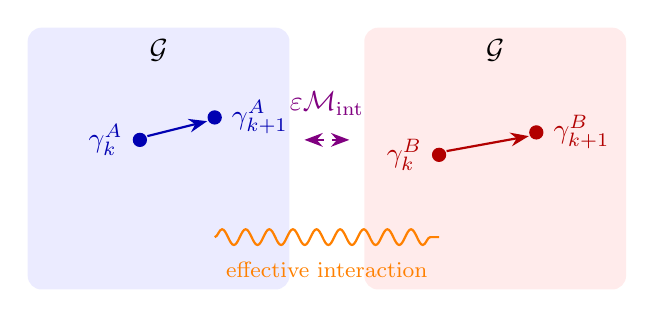
\begin{tikzpicture}[scale=0.95]
    % Two copies of G
    \fill[blue!8, rounded corners=5pt] (-4,-1.5) rectangle (-0.5,2);
    \fill[red!8, rounded corners=5pt] (0.5,-1.5) rectangle (4,2);
    \node at (-2.25,1.7) {$\Gspace$};
    \node at (2.25,1.7) {$\Gspace$};

    % gamma^A
    \filldraw[blue!70!black] (-2.5,0.5) circle (2.5pt);
    \node[blue!70!black, left] at (-2.6,0.5) {$\gamma^A_k$};
    \filldraw[blue!70!black] (-1.5,0.8) circle (2.5pt);
    \node[blue!70!black, right] at (-1.4,0.8) {$\gamma^A_{k+1}$};
    \draw[-{Stealth}, blue!70!black, thick] (-2.4,0.55) -- (-1.6,0.75);

    % gamma^B
    \filldraw[red!70!black] (1.5,0.3) circle (2.5pt);
    \node[red!70!black, left] at (1.4,0.3) {$\gamma^B_k$};
    \filldraw[red!70!black] (2.8,0.6) circle (2.5pt);
    \node[red!70!black, right] at (2.9,0.6) {$\gamma^B_{k+1}$};
    \draw[-{Stealth}, red!70!black, thick] (1.6,0.35) -- (2.7,0.55);

    % Coupling arrow
    \draw[{Stealth}-{Stealth}, thick, violet, dashed] (-0.3,0.5) -- (0.3,0.5);
    \node[violet, above] at (0,0.7) {$\varepsilon \Mfunc_{\mathrm{int}}$};

    % Effective interaction
    \draw[decorate, decoration={snake, amplitude=1mm, segment length=3mm},
          orange, thick] (-1.5,-0.8) -- (1.5,-0.8);
    \node[orange, below] at (0,-1) {\footnotesize effective interaction};
\end{tikzpicture}
\caption{Two-configuration system $(\gamma^A, \gamma^B) \in \Gspace \times \Gspace$.
Constraint coupling via~$\Mfunc_{\mathrm{int}}$ (dashed arrow) modifies
admissible evolution and produces an effective interaction (wavy line) in the IR.}
\label{fig:coupled-system}
\end{figure}

%-----------------------------------------------------------------------------
\subsection{Effective Interaction Potential}
\label{sec:effective-potential}
%-----------------------------------------------------------------------------

In the continuous-time limit, the coupled mismatch~\eqref{eq:coupled-mismatch}
yields an effective Lagrangian:
\begin{equation}
\label{eq:coupled-lagrangian}
L_{\mathrm{eff}} = \frac{1}{2} g^A_{ij} \dot{q}^{A,i} \dot{q}^{A,j}
+ \frac{1}{2} g^B_{ij} \dot{q}^{B,i} \dot{q}^{B,j}
- V_{\mathrm{int}}(q^A, q^B),
\end{equation}
where the effective interaction potential is
\begin{equation}
\label{eq:Vint}
V_{\mathrm{int}}(q^A, q^B) = \varepsilon \,
\lim_{\Delta \to 0} \frac{1}{\Delta} \Mfunc_{\mathrm{int}}.
\end{equation}

\begin{proposition}[Emergence of Effective Forces]
\label{prop:effective-forces}
The equations of motion derived from~\eqref{eq:coupled-lagrangian} are
\begin{equation}
\label{eq:coupled-eom}
\Meff^A \ddot{X}^A = -\nabla_{X^A} V_{\mathrm{int}}, \qquad
\Meff^B \ddot{X}^B = -\nabla_{X^B} V_{\mathrm{int}},
\end{equation}
in the translation sector, recovering the structure of interacting effective
particles.
\end{proposition}

%-----------------------------------------------------------------------------
\subsection{Reduction to the BP4/BP5 Two-Body Structure}
\label{sec:reduction}
%-----------------------------------------------------------------------------

In the weak-coupling and large-separation limit:
\begin{itemize}
    \item $|X^A - X^B| \gg \ell^A + \ell^B$ (configurations well-separated).
    \item $\varepsilon \ll 1$ (perturbative coupling).
\end{itemize}
The interaction potential~$V_{\mathrm{int}}$ reduces to the form derived in
BP4~\cite{BP4}:
\begin{equation}
\label{eq:Vint-BP4}
V_{\mathrm{int}}(X^A, X^B) \approx \kappa \, \frac{f(|X^A - X^B|)}{|X^A - X^B|^p},
\end{equation}
where $\kappa$ is a coupling constant and $f$, $p$ depend on the field theory
details. In the gravitational analogy sector, $p = 1$ and the Newtonian limit
is recovered.

%=============================================================================
\section{Conservation Laws from Symmetries of Admissibility}
\label{sec:conservation}
%=============================================================================

%-----------------------------------------------------------------------------
\subsection{Symmetry Assumptions}
\label{sec:symmetry-assumptions}
%-----------------------------------------------------------------------------

\begin{hypothesis}[Translation Invariance]
\label{hyp:translation}
The admissibility constraints are invariant under spatial translations: if
$\{\gamma_k\} \in \Adm$, then $\{T_a \gamma_k\} \in \Adm$ for any
$a \in \mathbb{R}^3$, where $T_a$ is the translation action.
\end{hypothesis}

\begin{hypothesis}[Time-Homogeneity]
\label{hyp:time-homog}
The constraints depend only on the relation between consecutive geometries,
not on the absolute step index~$k$.
\end{hypothesis}

%-----------------------------------------------------------------------------
\subsection{Emergent Conserved Quantities}
\label{sec:conserved}
%-----------------------------------------------------------------------------

\begin{proposition}[Momentum Conservation]
\label{prop:momentum}
Under Hypothesis~\ref{hyp:translation}, the total momentum
\begin{equation}
\label{eq:total-momentum}
P^i_{\mathrm{total}} = \sum_{\alpha} g^{\alpha}_{ij}(q^\alpha) \dot{q}^{\alpha,j}
\end{equation}
is conserved along admissible histories, up to corrections of order~$O(\varepsilon^2)$
from constraint coupling.
\end{proposition}

\begin{proof}
Translation invariance implies that $\Mfunc_{\mathrm{total}}$ depends only on
relative coordinates. The standard Noether argument applied to the effective
Lagrangian~\eqref{eq:coupled-lagrangian} yields momentum conservation.
Higher-order coupling corrections may introduce small non-conservation.
\end{proof}

\begin{corollary}[Energy Conservation]
\label{cor:energy}
Under Hypothesis~\ref{hyp:time-homog}, the effective energy
\begin{equation}
\label{eq:total-energy}
E_{\mathrm{total}} = \sum_{\alpha} \frac{1}{2} g^{\alpha}_{ij}
\dot{q}^{\alpha,i} \dot{q}^{\alpha,j} + V_{\mathrm{int}}
\end{equation}
is conserved along admissible histories in the continuous-time limit.
\end{corollary}

%=============================================================================
\section{Breakdown Regimes and Failure of Admissibility}
\label{sec:breakdown}
%=============================================================================

%-----------------------------------------------------------------------------
\subsection{When Constraints Cannot Be Satisfied}
\label{sec:failure}
%-----------------------------------------------------------------------------

The admissibility framework breaks down when the constraints
(Hypotheses~\ref{hyp:stability}--\ref{hyp:internal-mode}) cannot be simultaneously
satisfied. This occurs in several scenarios:

\paragraph{Stability Loss.}
If external perturbations or rapid evolution drive the configuration toward
the boundary of the stable manifold:
\begin{equation}
\Egeom(\gamma_k) \to E^*, \qquad
\delta^2 \Egeom|_{\gamma_k} \to 0,
\end{equation}
then admissible successors may not exist, signalling a phase transition or
decay of the configuration.

\paragraph{Internal Mode Excitation.}
If the evolution excites internal modes beyond the regularity bound:
\begin{equation}
\| P_{\mathrm{int}} \delta\gamma_k \| > \epsilon_{\mathrm{int}},
\end{equation}
the collective-coordinate description fails, and energy leaks into radiation
modes.

\paragraph{Reconstruction Lag.}
If the required rate of change exceeds what reconstruction can accommodate:
\begin{equation}
\Mfunc(\gamma_{k+1}, \gamma_k; \Rmap) > \Mfunc^*,
\end{equation}
no admissible successor exists, indicating that the evolution is too ``fast''
for the underlying field dynamics.

%-----------------------------------------------------------------------------
\subsection{Effective Description of Breakdown}
\label{sec:effective-breakdown}
%-----------------------------------------------------------------------------

Near but not at breakdown, corrections to the geodesic equations appear:

\begin{proposition}[Dissipative Corrections]
\label{prop:dissipative}
When internal modes are weakly excited, the effective equations of motion
acquire dissipative terms:
\begin{equation}
\label{eq:dissipative}
\Meff \ddot{X} + \eta \dot{X} = -\nabla V_{\mathrm{int}},
\end{equation}
where $\eta > 0$ is an effective damping coefficient arising from energy
transfer to internal modes.
\end{proposition}

This corresponds to radiation damping in the underlying field theory and
is consistent with the prediction structure of BP4~\cite{BP4}.

%=============================================================================
\section{Scope and Non-Claims}
\label{sec:non-claims}
%=============================================================================

To maintain the conservative posture of bridge papers, we explicitly state
what this framework does \emph{not} claim:

\begin{itemize}
    \item \textbf{Not a derivation of special or general relativity.}
          The framework is compatible with Lorentz invariance in the IR,
          but does not derive it from first principles.
    \item \textbf{Not a quantum theory.}
          All constructions are classical. Quantisation of the configuration
          space~$\Gspace$ is not addressed.
    \item \textbf{No claims about quantum measurement or collapse.}
    \item \textbf{Not a fundamental ontology.}
          This is an effective bridge description, not a claim about ultimate
          reality.
    \item \textbf{No consciousness or observer primacy.}
          ``Observer'' in this paper means only frame choice, coarse-graining,
          or boundary conditions---not conscious agents.
    \item \textbf{No preferred reference frame.}
    \item \textbf{No derivation of the Standard Model.}
          The field content is taken as given; we do not derive particle spectra.
\end{itemize}

%=============================================================================
\section{Conclusion}
\label{sec:conclusion}
%=============================================================================

This paper has recast dynamics as a selection problem on the configuration
space of stabilised geometries. Building on BP5's reconstruction interpretation
of motion, we defined admissibility constraints---stability, bounded mismatch,
internal mode regularity---that filter which histories are physically realised.
In the deep-stabilisation regime, admissible paths approximate geodesics on a
metric derived from the mismatch functional, recovering the effective mass and
inertial structure of BP4. Multi-configuration systems exhibit constraint coupling,
which yields effective interaction potentials in the infrared limit. Conservation
laws emerge from symmetries of the admissibility conditions.

A natural next step is the formulation of a path-integral or other quantisation
procedure on~$\Gspace$, which we defer to future work.

%=============================================================================
% APPENDICES
%=============================================================================
\appendix

\section{Discrete-to-Continuous Limit Derivation}
\label{app:discrete-continuous}

We derive the continuous-time limit of the mismatch functional and the
emergence of the moduli space metric.

\subsection{Setup}

Let $\gamma(t) \in \Gspace$ be a continuous history, discretised as
$\gamma_k = \gamma(k\Delta)$ for step size~$\Delta$. A representative
field configuration is $\Phi_0(x; q(t))$, where $q(t)$ are collective coordinates.

\subsection{Mismatch Expansion}

The reconstruction map $\Rmap_\Delta$ acts on field configurations. For small~$\Delta$,
we assume $\Rmap_\Delta[\Phi_0(q_k)] \approx \Phi_0(q_k) + O(\Delta)$, encoding that
reconstruction attempts to preserve the configuration.

The mismatch~\eqref{eq:mismatch} becomes:
\begin{align}
\Mfunc(\gamma_{k+1}, \gamma_k) &=
\inf_{\text{reps}} \int \dd^3x \,
\bigl| \Phi_0(x; q_{k+1}) - \Rmap_\Delta[\Phi_0(x; q_k)] \bigr|^2 w(x) \\
&\approx \int \dd^3x \,
\bigl| \Phi_0(x; q_k + \dot{q}_k \Delta) - \Phi_0(x; q_k) \bigr|^2 w(x) \\
&= \int \dd^3x \,
\left| \frac{\partial \Phi_0}{\partial q^i} \dot{q}^i \Delta \right|^2 w(x)
+ O(\Delta^3) \\
&= \Delta^2 \, g_{ij}(q) \dot{q}^i \dot{q}^j + O(\Delta^3),
\end{align}
where
\begin{equation}
g_{ij}(q) = \int \dd^3x \,
\frac{\partial \Phi_0}{\partial q^i} \frac{\partial \Phi_0}{\partial q^j} w(x).
\end{equation}

\subsection{Action Integral}

Summing over $N = T/\Delta$ steps:
\begin{align}
\sum_{k=0}^{N-1} \Mfunc(\gamma_{k+1}, \gamma_k)
&= \sum_{k=0}^{N-1} \Delta^2 \, g_{ij} \dot{q}^i \dot{q}^j + O(\Delta^2) \\
&= \Delta \sum_{k=0}^{N-1} \Delta \, g_{ij} \dot{q}^i \dot{q}^j + O(\Delta^2) \\
&\to \Delta \int_0^T \dd t \, g_{ij}(q) \dot{q}^i \dot{q}^j
\quad \text{as } \Delta \to 0.
\end{align}

Rescaling, the total mismatch cost is proportional to the kinetic action:
\begin{equation}
S_{\mathrm{kin}} = \frac{1}{2} \int_0^T \dd t \, g_{ij}(q) \dot{q}^i \dot{q}^j.
\end{equation}

Minimising this action yields the geodesic equation~\eqref{eq:geodesic-eqn}.

%-----------------------------------------------------------------------------
\section{Notation Summary}
\label{app:notation}

Table~\ref{tab:notation} summarises the notation used in this paper and its
relation to BP4/BP5.

\begin{table}[h]
\centering
\caption{Notation summary.}
\label{tab:notation}
\begin{tabular}{lll}
\hline
\textbf{Symbol} & \textbf{Meaning} & \textbf{BP4/BP5 relation} \\
\hline
$\Phi$ & Field configuration & Same as BP4/BP5 \\
$\Phi_0$ & Stabilised field configuration & Same as BP4/BP5 \\
$\Egeom$ & Geometric (gradient + potential) energy & Same as BP4 \\
$E_0$ & Ground state energy & Same as BP4 \\
$\Meff$ & Effective mass & Same as BP4 \\
$\kappa$ & Coupling constant & Same as BP4 \\
$X(t)$ & Collective coordinate (translation) & Same as BP4/BP5 \\
$\ell$ & Characteristic length scale & Same as BP4/BP5 \\
$\xi$ & Internal moduli & Same as BP5 \\
$\Gspace$ & Configuration space of stabilised geometries & New in BP6 \\
$\gamma$ & Element of $\Gspace$ & New in BP6 \\
$\Rmap_\Delta$ & Reconstruction map & From BP5 \\
$\Mfunc$ & Mismatch functional & From BP5 \\
$\Adm$ & Admissible region/set & New in BP6 \\
$g_{ij}$ & Moduli space metric & Implicit in BP4 \\
$\Mfunc^*$ & Mismatch threshold & New in BP6 \\
$E^*$ & Energy threshold for stability & New in BP6 \\
$\varepsilon$ & Interaction coupling strength & New in BP6 \\
$c$ & Speed of light & Same as BP4/BP5 \\
\hline
\end{tabular}
\end{table}

%=============================================================================
% FIGURE: BRIDGE PAPER ARC
%=============================================================================

\begin{figure}[ht]
\centering
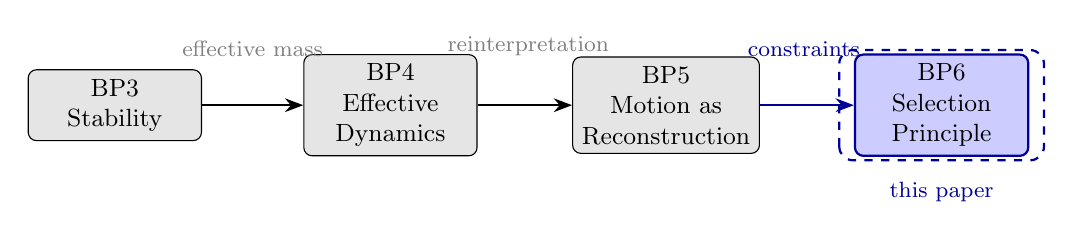
\begin{tikzpicture}[scale=1.0,
    box/.style={draw, rounded corners=3pt, minimum width=2.2cm,
                minimum height=0.9cm, align=center, font=\small}]

    % Boxes
    \node[box, fill=gray!20] (bp3) at (0,0) {BP3\\Stability};
    \node[box, fill=gray!20] (bp4) at (3.5,0) {BP4\\Effective\\Dynamics};
    \node[box, fill=gray!20] (bp5) at (7,0) {BP5\\Motion as\\Reconstruction};
    \node[box, fill=blue!20, thick, draw=blue!60!black] (bp6) at (10.5,0)
        {BP6\\Selection\\Principle};

    % Arrows
    \draw[-{Stealth}, thick] (bp3) -- (bp4);
    \draw[-{Stealth}, thick] (bp4) -- (bp5);
    \draw[-{Stealth}, thick, blue!60!black] (bp5) -- (bp6);

    % Labels
    \node[above, font=\footnotesize, gray] at (1.75,0.5) {effective mass};
    \node[above, font=\footnotesize, gray] at (5.25,0.5) {reinterpretation};
    \node[above, font=\footnotesize, blue!60!black] at (8.75,0.5) {constraints};

    % Highlight
    \draw[blue!60!black, thick, dashed, rounded corners=5pt]
        (9.2,-0.7) rectangle (11.8,0.7);
    \node[blue!60!black, font=\footnotesize] at (10.5,-1.1) {this paper};
\end{tikzpicture}
\caption{Bridge paper arc from BP3 to BP6. BP6 elevates the reconstruction
interpretation (BP5) to a selection principle via admissibility constraints.}
\label{fig:bp-arc}
\end{figure}

%=============================================================================
% BIBLIOGRAPHY
%=============================================================================
\bibliographystyle{plain}
\bibliography{refs}

\end{document}
